\chapter{Reflectie en discussie}
In dit laatste hoofdstuk zullen we een analyse maken van het praktische deel van ons project.

Wanneer we kijken naar de grafieken, wordt het direct duidelijk dat de Fouriertransformatie in eigenlijk alle gevallen een slechter resultaat oplevert. Er is zowel een subjectieve `wolligheid' die geassoci\"eerd kan worden met het verlies
van details als een objectief verschil in PSNR. Het enige geval waarin Fourier echt beter presteert dan de wavelets is wanneer we kijken naar een periodieke functie.
\begin{figure}[h]
  \centering
  \begin{subfigure}[b]{0.25\textwidth}
    \centering
    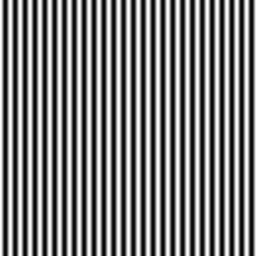
\includegraphics[width=\textwidth]{plaatjes/sin_fourier.png}
  \end{subfigure}
  \begin{subfigure}[b]{0.25\textwidth}
    \centering
    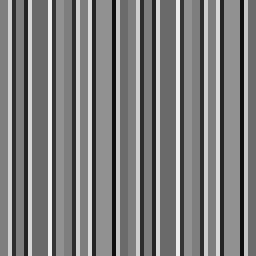
\includegraphics[width=\textwidth]{plaatjes/sin.png}
  \end{subfigure}
  \caption{Een periodiek signaal wordt perfect door de Fouriertransformatie gereconstrueerd bij 1 \% van de data, maar de wavelettransformatie kan op het zelfde niveau niet tippen.}
\end{figure}

De reden hiervoor is al veelvuldig aangedragen: waveletbasisfuncties hebben een lokale drager, terwijl de basisfuncties van Fourier op de hele ruimte werken. Hoewel dit een heel voor de hand liggende reden is, is het toch mooi om dit in de praktijk te zien.

\section{Discussie}
\subsection{Gebruik van PSNR als maatstaf voor kwaliteit}
Omdat we te maken hebben met `lossy' beeldcompressie dienen we dit verlies in kaart te brengen op een 
objectieve en kwantitatieve manier. 
De PSNR is een gebruikelijke grootheid voor dit soort analyses, er wordt gezegd dat dit voor eenzelfde 
beginsignaal een goede reflectie geeft van de menselijke beleving van de kwaliteit van de reconstructie.
We beroepen ons hier dan ook op de ander onderzoek NEEDS MOAR REFS

\section{Fotorealisme versus strak}
Kijkende naar Lenna op de verschillende compressieniveaus, is het duidelijk dat de Daubechieswavelet bla
